\section{Comparing the results of the first user journey}\label{section:results:comparison-first-journey}

This section describes how the shared caching layer and the reduction of queries were tested for the prototypical micro-frontend architecture. It explains the first user journey through the application and shows the three approaches results. Figure \ref{fig:results:evaluation-first-path} shows the steps through the micro-frontend prototype used to measure the possible performance improvements of the shared caching layer and the reduction of queries. The client has to perform 13 steps throughout the application, which involves almost every available GraphQL query. The dashboard micro-frontend yields some problems if the evaluation is started there. All widgets are created and start to fetch their data simultaneously. Therefore, it can easily happen that multiple widgets fetch the same queries from the GraphQL \ac{API} because the data is not already in the cache. This problem leads to a lot of theoretically unnecessary network requests and is difficult to circumvent. The evaluation shown in the figure is performed with an unauthenticated user. And this section takes the measurements and compares the different approaches regarding request sizes and response sizes, the number of requests, and the total records fetched.

\ifshowImages
\begin{figure}[H]
\centering
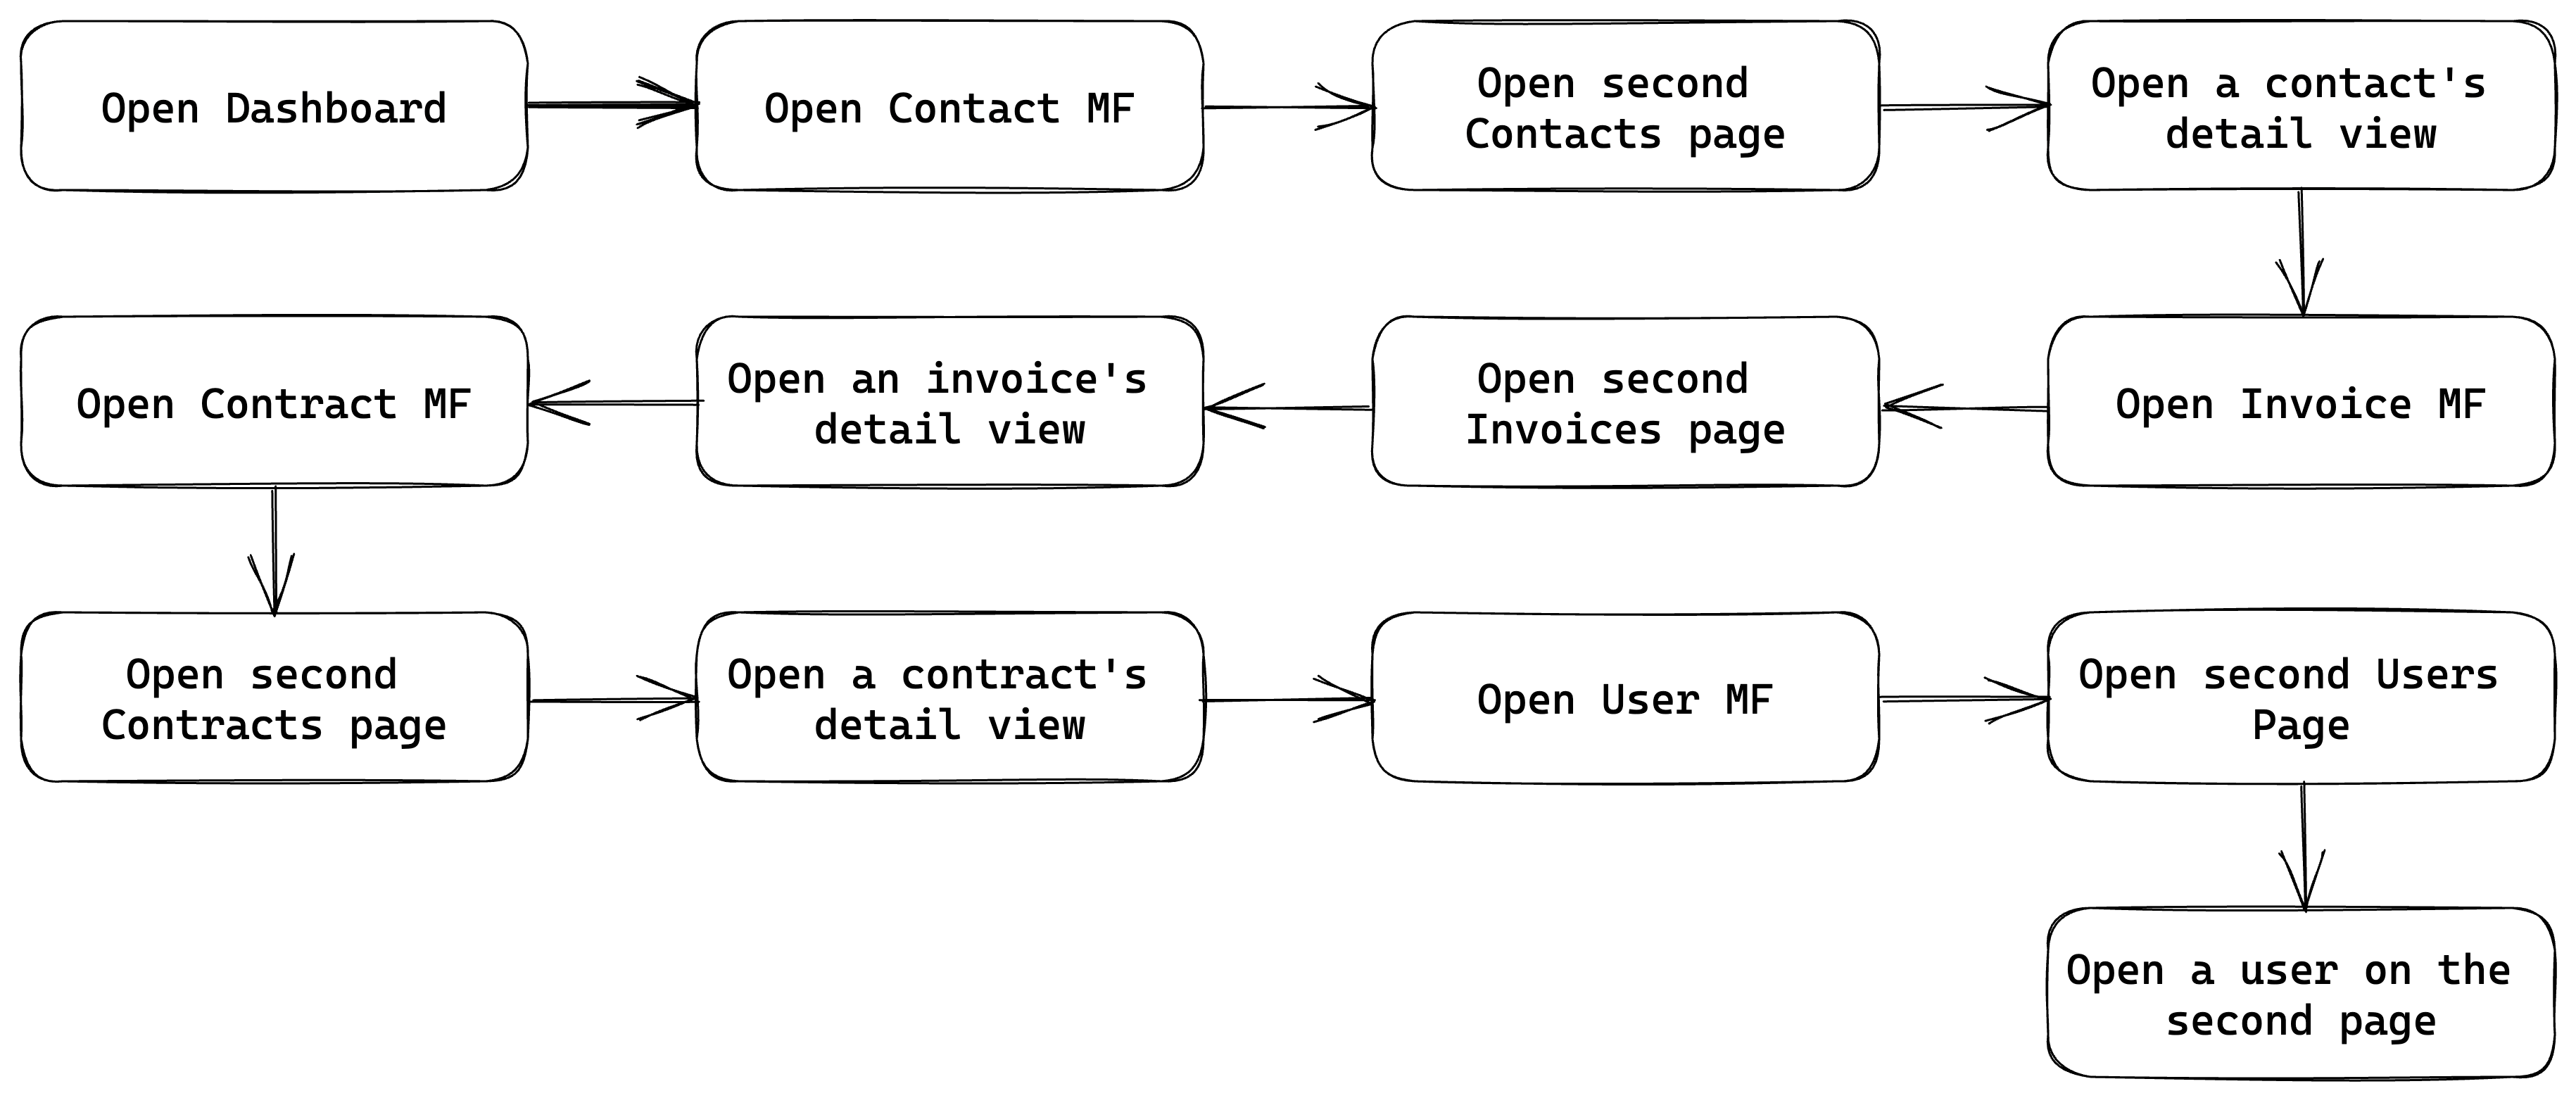
\includegraphics[width=1\linewidth]{images/results/evaluation-first-path.png}
\caption{A user journey through the application to measure the performance of the micro-frontend architecture.}\label{fig:results:evaluation-first-path}
\end{figure}
\fi

\noindent Without a caching system, the GraphQL \ac{API} would have to run 59 queries to provide the data for the journey through the application. How the prototypical micro-frontend architecture can be configured to use one of the three approaches is already explained in Section \ref{section:applied-methods:shared-caching-layer} and Section \ref{subsection:applied-methods:query-reduction:testing-query-reduction}. The following sections describe and compare the results of the approaches in more detail.

\subsubsection{Separate Cache and no reduced queries}\label{subsubsection:results:performance-measurement:separate-cache-no-reduction}

With this approach, each micro frontend has a separate instance of the GraphQL client and \texttt{InMemoryCache}. The queries are not reduced using the cache and the custom implementation. After the client completes the journey through the application, the following metrics are collected.

\begin{itemize}
  \item 47 network requests to the GraphQL \ac{API}
  \item 10.80 MB transferred (request size + response size)
\end{itemize}

\noindent The \texttt{GRAPHQL\_CLIENT\_OPTIONS\_CONFIG} and \texttt{REDUCE\_QUERY\_OPTIONS} injection tokens have to be configured the following way. A more detailed description of the configuration options can be found in Section \ref{section:applied-methods:shared-caching-layer} and in Section \ref{subsection:applied-methods:query-reduction:testing-query-reduction}:

\begin{itemize}
  \item \texttt{shareCache: false}
  \item \texttt{reduceQueries: false}
\end{itemize}

\noindent 47 network requests have to be made to the GraphQL \ac{API}, which can be seen in Figure \ref{fig:results:no-shared-cache-no-reduction}. The figure shows 54 requests, but 7 requests have to be subtracted because they are needed to make the prototypical architecture work. They load the micro-frontends from their remote locations and fetch their settings, and these requests are only needed for the functionality of the micro-service architecture

\ifshowImages
  \begin{figure}[H]
  \centering
  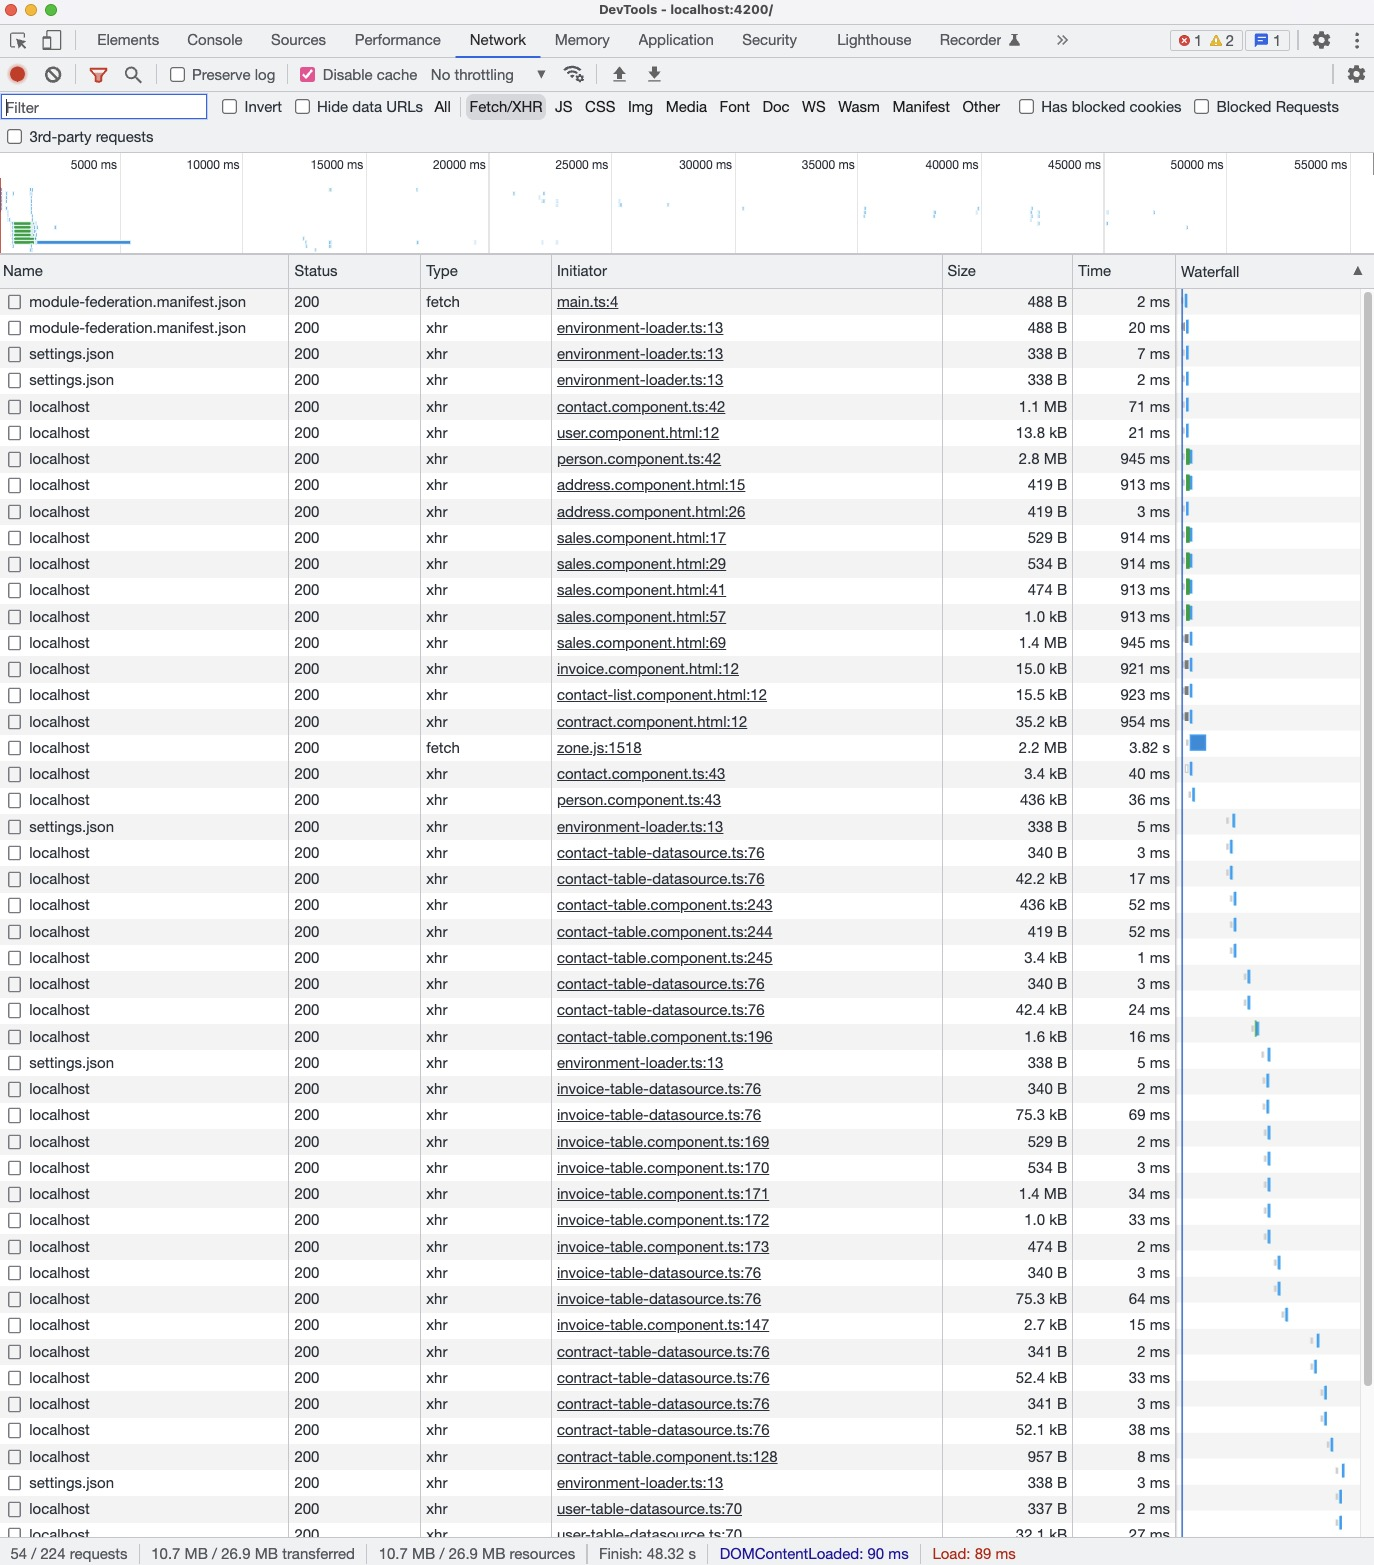
\includegraphics[width=0.75\linewidth]{images/results/1-attempt/no-shared-cache-no-reduction.jpg}
  \caption{All requests made during the measurement of the first approach.}\label{fig:results:no-shared-cache-no-reduction}
\end{figure}
\fi

\noindent The total size of the requests was 17.46 KB, and the responses were 10.78 MB. The 47 queries retrieve a total of 81510 records from the GraphQL  \ac{API}.

\subsubsection{Shared Cache and no reduced queries}\label{subsubsection:results:performance-measurement:shared-cache-no-reduction}

With this approach, an instance of the cache is shared by all micro-frontends, but the GraphQL queries are not reduced with data already present in the \texttt{InMemoryCache}. After the client completes the journey through the application, the following metrics are collected:

\begin{itemize}
  \item 36 network requests to the GraphQL \ac{API}
  \item 8.45 MB transferred (request size + response size)
\end{itemize}

\noindent The \texttt{GRAPHQL\_CLIENT\_OPTIONS\_CONFIG} and \texttt{REDUCE\_QUERY\_OPTIONS} injection tokens have to be configured the following way:

\begin{itemize}
  \item \texttt{shareCache: true}
  \item \texttt{reduceQueries: false}
\end{itemize}

\noindent 36 requests have to be made to the GraphQL \ac{API}, which can be seen in Figure \ref{fig:results:shared-cache-no-reduction}. Seven requests have to be deducted (\texttt{settings.json}, \texttt{module-federation.manifest.json}, \dots) as in the previous section.

\ifshowImages
  \begin{figure}[H]
  \centering
  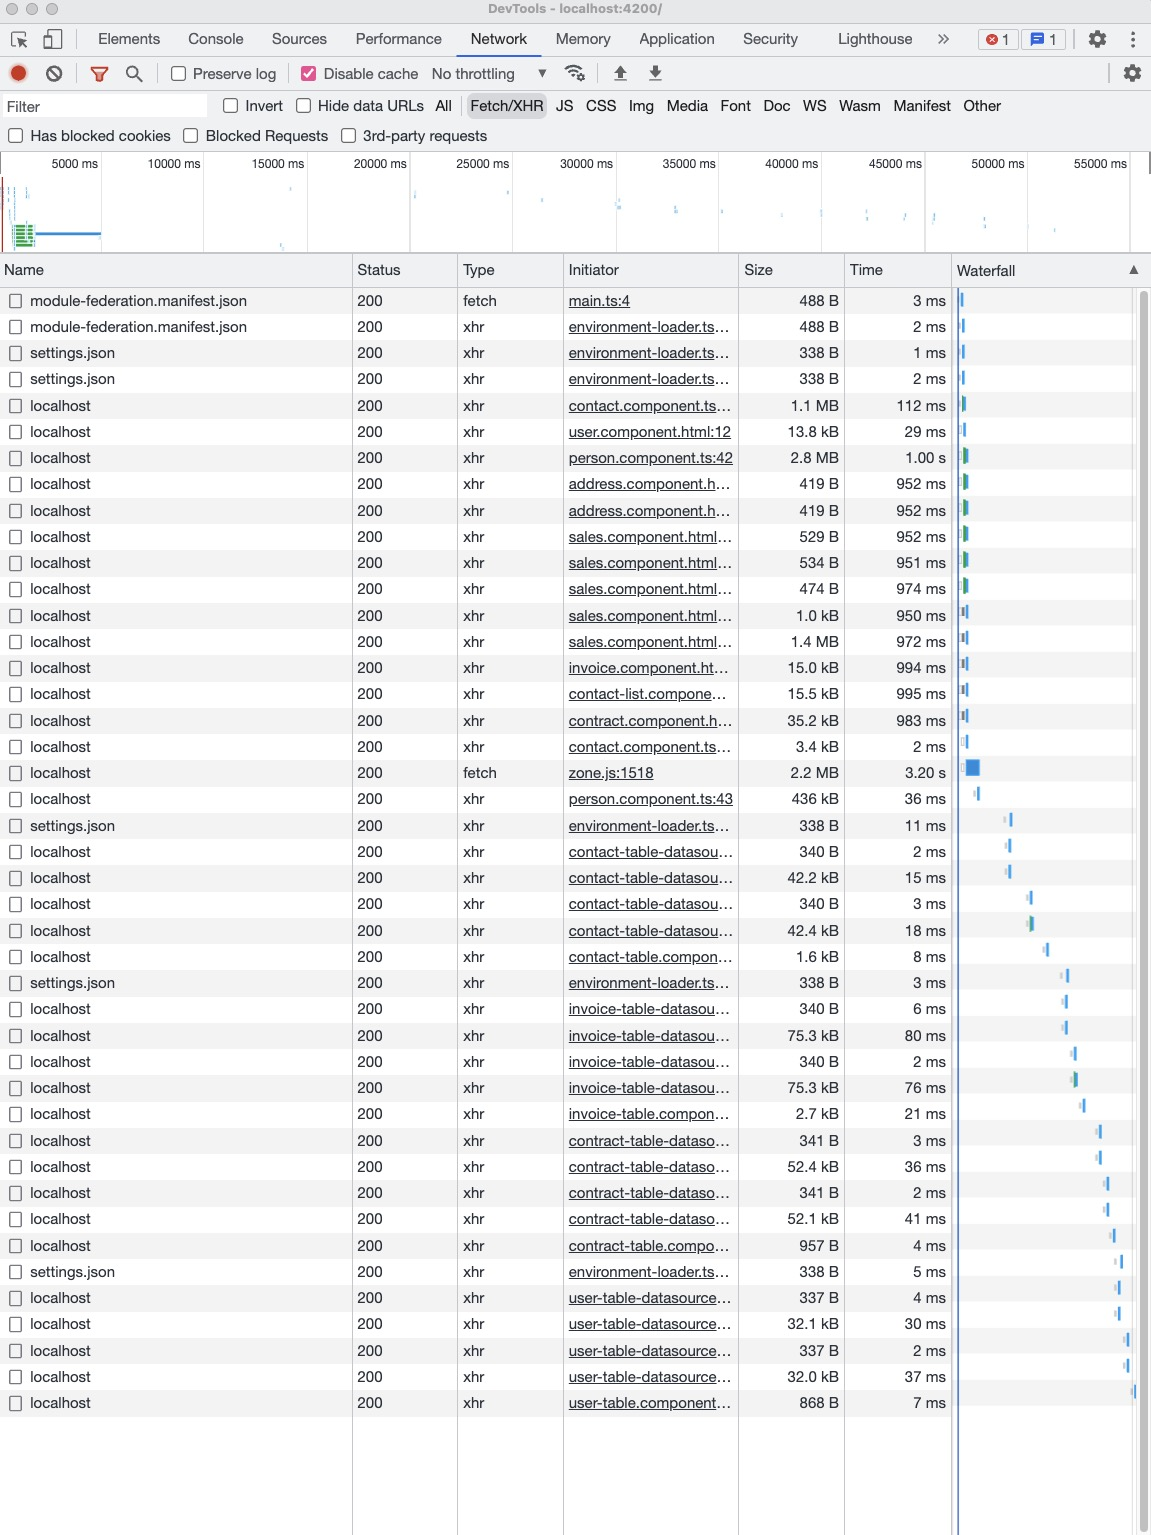
\includegraphics[width=0.75\linewidth]{images/results/1-attempt/shared-not-reduced-cache.jpg}
  \caption{All requests made during the measurement of the second approach.}\label{fig:results:shared-cache-no-reduction}
\end{figure}
\fi

\noindent The total size of the queries was 15.18 KB, and the size of the responses was 8.43 MB. The 36 queries retrieve a total of 51319 records from the GraphQL \ac{API}.

\subsubsection{Shared cache, query reduction}\label{subsubsection:results:performance-measurement:separate-cache-reduction}

With this approach, the same instance of the cache is shared between all of the micro-frontends in the architecture, and the queries are reduced with already existing data inside the cache. After the client completes the journey through the application, the following metrics are collected.

\begin{itemize}
  \item 36 network requests to the GraphQL \ac{API}
  \item 8.39 MB transferred (request size + response size)
\end{itemize}

\noindent The \texttt{GRAPHQL\_CLIENT\_OPTIONS\_CONFIG} and \texttt{REDUCE\_QUERY\_OPTIONS} injection tokens have to be configured the following way:

\begin{itemize}
  \item \texttt{shareCache: true}
  \item \texttt{reduceQueries: true}
\end{itemize}

\noindent 36 requests have to be made to the GraphQL \ac{API}, which can be seen in Figure \ref{fig:results:shared-cache-reduction}. Seven requests have to be deducted (\texttt{settings.json}, \texttt{module-federation.manifest.json}, \dots) as in the previous sections.

\ifshowImages
  \begin{figure}[H]
  \centering
  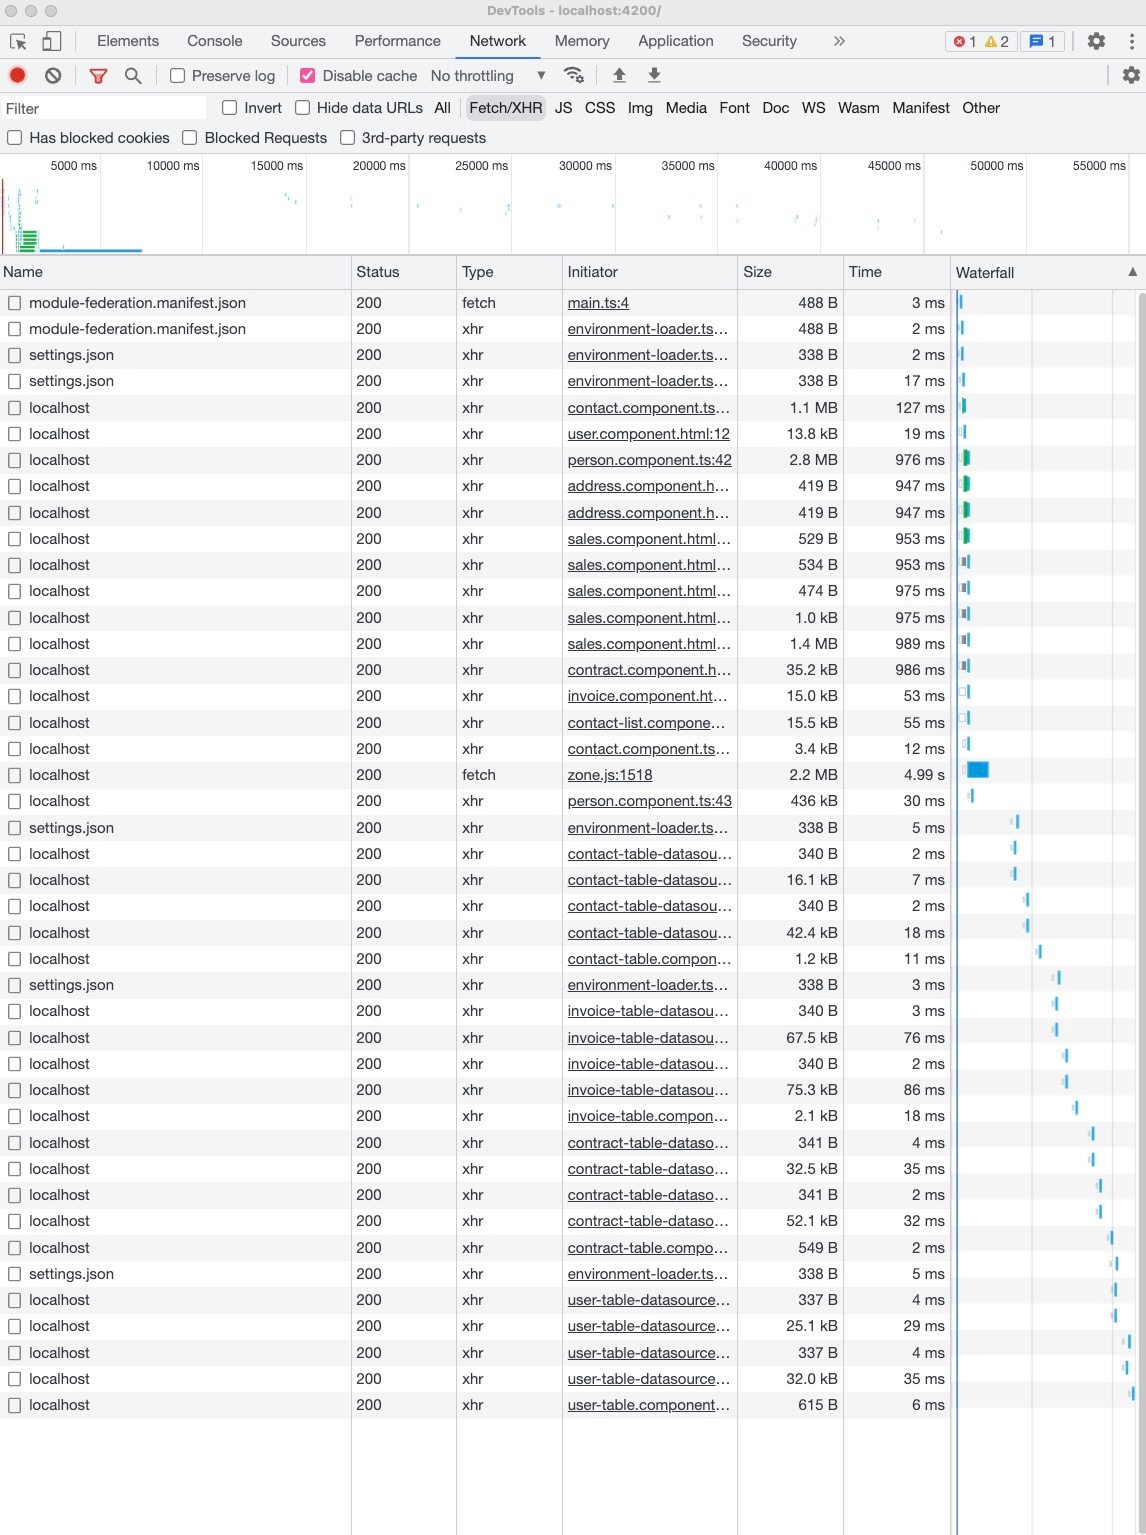
\includegraphics[width=0.75\linewidth]{images/results/1-attempt/shared-reduced-cache.jpg}
  \caption{All requests made during the measurement of the third approach.}\label{fig:results:shared-cache-reduction}
\end{figure}
\fi

\noindent The total size of the queries was 13.53 KB, and the size of the responses was 8.37 MB. The 36 queries retrieve a total of 51319 records from the GraphQL \ac{API}.

\subsection{Comparing the first- and second-approach}\label{subsection:results:comparison-first-second-approach}

When comparing the first- with the second approach, there is a significant difference in the number of network requests made to the GraphQL \ac{API} and the size of the requests and responses, as seen in Table \ref{table:results:size-comparison-first-path-no-cache-no-reduction-cache-no-reduction}. The shared cache approach requires eleven fewer network requests than the separate cache approach. Since the queries are not reduced for this comparison, the additional network queries account for the overall difference in request- and response size. The 11 additional requests from the first approach send an additional 2.29 KB to the \ac{API} and return about an additional 2.34 MB from the \ac{API}. Therefore, 22\% of the total response size can be saved using only one shared cache for all micro-frontends. Another interesting observation is that the shared cache approach retrieves 30191 fewer records than the naive approach, about 37\% of the total records returned.

\ifshowTables
\begin{table}[H]
  \begin{tabular}{|l|l|l|l|l|}
  \hline
    & \textbf{Req. Size (B)} & \textbf{Resp. Size (B)} & \textbf{Requests} & \textbf{Records} \\
    \hline
    \textbf{No Reduction, Separate Cache} & 17462 & 10780656 & 47 & 81510 \\
    \hline
    \textbf{No Reduction, Shared Cache} & 15176 & 8437211 & 36 & 51319 \\
    \hline
    \hline
    \textbf{Diff} & \textbf{2286} & \textbf{2343445} & \textbf{11} & \textbf{30191} \\
    \hline
    \textbf{Reduction (\%)} & \textbf{13\%} & \textbf{22\%} & \textbf{23\%} & \textbf{37\%} \\
    \hline
  \end{tabular}
  \caption{First Journey: Compare the requests and responses of the first- and second-approach.}\label{table:results:size-comparison-first-path-no-cache-no-reduction-cache-no-reduction}
\end{table}
\fi

\noindent The following enumeration shows which and how often GraphQL queries were dropped when using a shared caching layer between the micro front-ends compared to a separate cache:

\begin{itemize}
  \item allCountries: 2
  \item allSalutations: 2
  \item allTitles: 2
  \item allArticleUnits: 1
  \item allCurrencies: 1
  \item allVats: 1
  \item allSalesCountries: 1
  \item allInvoiceTypes: 1
\end{itemize}

\noindent The data of the omitted requests is usually used for filling selection controls inside detail views and has to be fetched repeatedly in every micro-frontend. The first three queries are used for widgets on the dashboard, the contact application, and the user application. The last five queries are used for widgets on the dashboard and the sales application.

\subsection{Comparing the first- and third-approach}\label{subsection:results:comparison-first-third-approach}

As in the previous comparison, there is the same difference in the number of network requests made to the GraphQL \ac{API}. The size of the responses and the requests have a massive difference, just like before. The results are shown in Table \ref{table:results:size-comparison-first-path-no-cache-no-reduction-cache-reduction}. Just like before, there is a difference of 11 GraphQL queries that are sent to the GraphQL \ac{API}. However, due to the reduction in queries, the difference in the size of the queries and responses is greater than in Section \ref{subsection:results:comparison-first-second-approach}. All queries of the first approach send 3.92 KB more and return about 2.41 MB more from the GraphQL \ac{API} compared to the third approach. A shared cache and query reduction can save about 22\% response sizes. As before, 37\% fewer records need to be fetched from the \ac{API}.

\ifshowTables
\begin{table}[H]
  \begin{tabular}{|l|l|l|l|l|}
  \hline
  & \textbf{Req. size (B)} & \textbf{Resp. size (B)} & \textbf{Requests} & \textbf{Records}  \\
  \hline
  \textbf{No Reduction, Separate Cache} & 17462 & 10780656 & 47 & 81510 \\
  \hline
  \textbf{Reduction, Shared Cache} & 13533 & 8374763 & 36 & 51319 \\
  \hline
  \hline
  \textbf{Diff} & \textbf{3929} & \textbf{2405893} & \textbf{11} & \textbf{30191} \\
  \hline
  \textbf{Reduction (\%)} & \textbf{23\%} & \textbf{22\%} & \textbf{23\%} & \textbf{37\%} \\
  \hline
  \end{tabular}
  \caption{First Journey: Compare the requests and responses of the first- and third-approach.}\label{table:results:size-comparison-first-path-no-cache-no-reduction-cache-reduction}
\end{table}
\fi

\subsection{Comparing the second- and third-approach}\label{subsection:results:comparison-second-third-approach}

Between the first and second approaches, there is almost no difference in request- and response size compared to the comparisons from sections \ref{subsection:results:comparison-first-second-approach} and \ref{subsection:results:comparison-first-third-approach}, as seen in Table \ref{table:results:size-comparison-first-path-cache-no-reduction-cache-reduction}. Both approaches have the same number of queries sent to the GraphQL \ac{API} since all micro-frontends share the same cache instance. Reducing queries does not lead to fewer network requests, because it just removed fields from executed queries. The difference in request and response size between the two approaches comes solely from query reduction. Using the third approach, the difference in request size is about 1.64 KB (11\%), which is insignificant. The difference between the response sizes (62.45 KB) is almost zero in relation to the amount of data that was returned.

\ifshowTables
\begin{table}[H]
  \begin{tabular}{|l|l|l|l|l|}
  \hline
  & \textbf{Req. size (B)} & \textbf{Resp. size (B)} & \textbf{Requests} & \textbf{Records} \\
  \hline
  \textbf{No Reduction, Shared Cache} & 15176 &  8437211 & 36 & 51319 \\
  \hline
  \textbf{Reduction, Shared Cache} &  13533 &  8374763 & 36 & 51319 \\
  \hline
  \hline
  \textbf{Diff} & \textbf{1643} & \textbf{62448} & \textbf{0} & \textbf{0} \\
  \hline
  \textbf{Reduction (\%)} & \textbf{11\%} & \textbf{1\%} & \textbf{-} & \textbf{-} \\
  \hline
  \end{tabular}
  \caption{First Journey: Compare the requests and responses of the second- and third-approach.}\label{table:results:size-comparison-first-path-cache-no-reduction-cache-reduction}
\end{table}
\fi